\chapter{Theory}
	Pipeline inspection are a complex problem and include many engineering diciplines.
	This chapter introduces some of the basics about pipeline inspections when
	designing a guidance system capable of pipeline inspection. Basics on the mathematical model for
	\hugin will treated, together with some theory on how to model a camera view and how
	movement of points are described in the camera view.

\section{Pipeline Inspection Fundamentals}
	
	
	To include the right sensors are an important aspect of making an AUV follow a pipeline. There are
	different sensors available which can be suited for this purpose. First the Multibeam Echosounder
	(MBE). Usually a Echosounder emits one beam of sound and measures the time of travel of the sound
	beam. A multibeam echosounder emits a fan of sound beams which can be used to map a larger area around
	the vessel.

	A Side Scan Sonar are another practical sensor which could be useful. The Side Scan Sonar sends sound
	waves in the horizontal direction and provides good sensor data of the bottom around 200-300 meters in
	the horizontal direction. This sensor are usefull for initially finding the pipeline. A side scan
	sonar picture of a pipeline gives very distinct shadows and are easily detected. 

	
\section{Different Methods for Pipeline Following Discussed in Literature}
	A literature study was performed to see what other people have accomplished on the subject on AUV and 
	pipeline following. 
	
	****************************************MORE****************************
	\cite{piscis} describes briefly a prototype AUV equipped with a camera and sonar to carry out pipeline
	inspection missions. The AUV uses controllers for heading, speed and depth and visual guidance to
	follow the pipeline. 
	
	\cite{GuidanceReview} proposes to use a two-stage guidance problem. When submerging and ascending to the surface, 
	the AUV uses a LOS guidance law at full speed. When the pipeline is acquired the guidance law is
	switched to a visual guidance scheme, which allows for a precise guidance over the subsea cable or
	pipeline. 
		
	In \cite{MPC_pure_pursuit} a guidance system using Model Predictive Control (MPC) and PNG law was used to make 
	a guidance system able to track cables and pipelines on the sea bed using Doppler Velocity Log and Electro-
	Magnetic sensors to find the cable/pipeline. The report utilises the pure pursuit scheme, similar to what 
	predators do when they are hunting the pray. The cable/pipeline and AUV is formulated as moving points
	with mass. The engages in a tail chase with the pipeline ``point'', but the AUV never catches up with it. This 
	method is robust to model uncertainties and handles constraints of the vessel in a systematic way. The
	controller however shows problems when a current are introduced in the system. The AUV drifts of the 
	pipeline, but catches up with the waypoints in the end. This is due to the fact that the guidance
	system are in a pursuit with the pipeline and the trajectory the AUV follows are not important. The
	guidance system only tries to catch up with the pipeline ``point''.
	
	In \cite{Visual_inpsection_of_seabottom_by_AUV} a visual guidance system for inspection of underwater
	structures is presented. The visual system uses an Extended Kalman Filter to smooth and predict where 
	the structure i.e. pipeline will move in the next sample interval of for the image processing software. 
	A three dimensional model of the scene is constructed which then allows the guidance system to calculate 
	an input to the controllers.
	
	\cite{reactive_control_AUV} proposes a reactive control approach to pipeline tracking together with a 
	profiling sonar. Reactive control originated from the field of obstacle avoidance in autonomous land and air 
	vehicles. It uses \textit{Deformed Virtual Zones} (DVZ) which describes the interaction between the AUV and 
	the pipeline. The controller tries to minimise the deformation of the DVZ and calculates a feasible
	control input. The DVZ in this case is a prism with a cylindrical cavity directly underneath the AUV. If the AUV
	moves away from the pipeline the DVZ will be deformed and the controller will try to counteract the 
	motion. This is a computational inexpensive way of achieving a good pipeline following. This 
	method shows promising results but has yet to be implemented and tested in real-life scenarios. 
	
	In \cite{fuel_optimal_control} a fuel-optimal tracking controller is derived to minimise the fuel
	consumption of the AUV. It uses the fact that the least fuel consuming path is the shortest one. This
	paper derives a fuel optimal controller using the estimated fuel consumption as a minimisation index. 

	\cite{side_scan_sonar} describes two techniques for detecting and tracking pipelines using Side Scan
	Sonar and Multi-Beam Echosounders. Prior knowledge about the pipeline are utilised for the recognition
	of the pipeline. A pipeline creates very distinct shadows in a side scan sonar image and are easy to
	separate from the sea bottom.



\section{Reference systems}
	Movement must be described relative to something. This is the task of the reference systems. There are
	4 important reference system. The ECI (Earth Center Inertial) which is a truly inertial reference
	frame, i.e. it is not accelerating. Its axis are pointing through the north pole and through the
	equatorial line of the Earth fixed toward stationary points in space, the center is as the name
	suggests in the center of the Earth. 
	
	ECEF (Earth-Center Earth-Fixed) is another reference frame. It is defined as the ECI coordinate
	system, but this frame is rotatiting with the earths rotiaton rate. Which means that this frame is not
	strictly inertial, but the angular velocity of the Earths rotation are considered very small, and can
	be neglected compared to other velocities in the same frame. Position on the earth are described by
	\textit{longitude} and \textit{latitude}.

	An important reference frame when considering local motion are the NED (North East Down) frame. This
	frame is defined as the tangent plane on the current position, and moving with the object. The axis
	are pointing towards north, east and down. This frame can be used in local, and small areas, but are
	not valid for intercontinental travel. This frame will primarily be used in this report. 

	The last but important frame are the Body frame, which is the local frame of the object of interest.
	The body frame are defined as the x-axis along its forward movment, y-axis to the right of the movment
	direction, and the last pointing downward, to complete the right-hand system. This frame are
	convenient when defining velocities, forces and moments.
	

\section{Hydrodynamic Model}
	\label{sec:ch1-model}
	An Autonomous Underwater Vehicle is a complex, non-linear and coupled process. The model which is used in this
	report uses the 6 DOF model described in \cite{fossen}.
	\begin{equation}
	\label{eq:ch1-model}
		\begin{aligned}
			\mathbf{\dot{\eta}} &= \rotation \mathbf{\nu} \\
			\mass + \coriolis + \damping + \restoring &= \force \\
		\end{aligned}
	\end{equation}
	where 
	\begin{align*}
		\mathbf{\eta} &= [N \: E \: D \: \phi \: \theta \: \psi ]^T \\
		\mathbf{\nu}  &= [u \: v \: w \: p \: q \: r]^T \\
		\force & \in \mathbb{R}^6
	\end{align*}
	The Equation \eqref{eq:ch1-model} describes the kinematics and kinetics for the model. It is in the 
	mathematical sense just a Mass-damper-spring system. The Coriolis term, $\mathbf{C}(\mathbf{\nu})$,
	is a skew-symmetric matrix appering because the dynamics are formulated in a non-inertial frame.

	The $\damping$ matrix are the damping forces, including drag from the surrounding water. $\restoring$
	are the restoring forces acting on the AUV. The gravity and bouyancy forces are represented by
	six-dimentional vector.
	
	The $\rotation$ matrix is the rotation matrix of Euler coordinates which relates the velocity of the 
	vessel to actual movement in the NED reference system.




\section{Camera theory}
	\label{ch1-cameramodel}
	The camera properties or parameters can be divided into two categories; the intrinsic parameters and
	extrinsic parameters. The intrinsic parameters are constant parameters and vary from camera to camera.
	It is the focus distance and image distortion of the pixels away from the centre of the camera. 
	The extrinsic parameters relate the position of the point relative to camera coordinates. 
	These parameters are of course dependant on the position of the camera and change with time. 	This imply that 
	coordinates of a 2D point in the camera have to be transformed into a 3D point which can be used 
	by the control system on board the AUV. Since 
	we are going from less knowledge about a point to more knowledge about a point, some things are needed to be 
	estimated or measured to gain the ability to solve the 2D to 3D problem exactly.\cite{robotbok}

	Suppose a point in the world reference system, denoted by, $P_w \in \mathbb{R}^3$. The same point
	represented in the camera frame, $P_c$ are related to $P_w$ by a rotation matrix, $\mathbf{R} \in
	SO(3)$. This gives the following equation: 
	\begin{equation}
		P_w = \mathbf{R} P_c + O(t)
	\end{equation}
	where $O(t)$ is the origin of the camera frame. This means that the point in the camera view is
	described by the equation
	\begin{equation}
		\label{eq:ch1-P_c}
		\begin{aligned}
			P_c &= \mathbf{R}^T (P_w - O(t)) \\
			\mathbf{R}^T &= \mathbf{R}^{-1} 
		\end{aligned}
	\end{equation}

	A pinhole camera model are used to capture $P_c$ to image coordinates, $P_i \in
	\mathbb{R}^2$. 
	The principle behind a pinehole camera is that all lightbeams passes through a
	infinitesmall hole, or point, located in the origin of the camera frame.   
	\begin{figure}[hbtp]
		\centering
		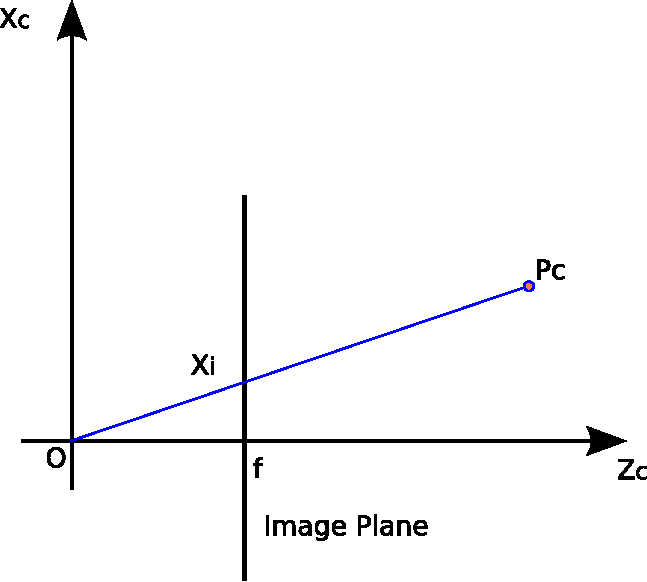
\includegraphics[width=0.6\textwidth]{pics/pinhole_model}
		\caption{Pinhole Camera Model showing two dimentions}
		\label{fig:ch1-pinhole}
	\end{figure}
			
	As seen from Figure \ref{fig:ch1-pinhole} the image plane is located a distance $f$ from the image plane. 
	The point is projected through the hole an onto the image plane. The principal axis of the camere is located
	in the direction of the observed point. For simplicity the image plane are located in the front of the
	pinhole, this is just in theory and is not possible in real camera application. From this the
	perspective equations are derived. \cite{robotbok}
	\begin{equation}
		\label{eq:ch1-perspective}
		P_i = \left[ \begin{array}{cc}
					\frac{f}{z_c} & 0 \\
					0	& \frac{f}{z_c} 
				\end{array} \right] 
				\left[ \begin{array}{c}
					x_c \\
					y_c
					\end{array} \right]
	\end{equation}
	This are the perspective equations which gives the observed point in screen coordinates. 

\section{Kalman filter}
	Kalman filtering a powerful and versatile tool in estimation and sensor fusion. A Kalman filter is
	usually employed in navigation applications to fuse GPS and INS together. By this way one will have
	the speed and resolution of an INS system and the precision of the GPS system.
	
	The Kalman Filter an optimal filter can be employed allmost in any application. It is optimal in 
	the sense of providing the minimum-variance estimate of the predicted prosess.  The Kalman 
	filter is a linear filter, and can only
	guarantee optimality for linear systems. There is a nonlinear version of the Kalman filter, the
	Extended Kalman Filter, which uses the same assumptions as the linear version but uses the nonlinear
	model to predict the state forward while it used a linearised version of the measurement equation. 
	When updating the Covariance matrix the system equations are linearised around the current estimate 
	and updated according to certain update laws. 
	
	********************MER INFO**************
	This introduces
	some significant problems. First the filter might converge towards wrong values, because of a 
	non-positive-definite covariance matrix. This is mostly due to poor linearisation of the state 
	equations. \cite{kalman}
	
\section{Guidance}
        \label{chap1-guidance-alg}
	Most of the guidance algorithms originates from airborne missile systems. This have been well
	documented and proven to work in numerous cases. Common guidance schemes such as Line-of-sight (LOS)
	and Proportional Navigation Guidance (PNG) and various implementations of these are employed in
	numerous guidance systems. 
	
	Guidance are defined according to \cite{guidance_def}
	\begin{definition}
		\label{def:ch1_guidance}
		The process of guiding the path of an object towards a given point, which in general may be
		moving.
	\end{definition}
	It is also convenient to define two levels of guidance.
	\begin{definition}
		The process of making an object converge geometrically to a given point or path is known as
		path following.
	\end{definition}
	\begin{definition}
		The process of making an object follow a gemoetric path with given dynamical constraints
		possibily dependant on position and time at the given path is known as trajectory tracking.
	\end{definition}
	The guidance systems discussed later will concern the first problem. The second problem will be
	disregarded and assumed that the dynamical constraints are constant and met. \cite{guidance-path-2d-3d}

	The guidance system need to adress the importance of a optimal paths. Optimal in the sense
	of energy consumption. A guidance system should be able to give 
	feasible commands to the lower level control system which controls the actuators, and should be able
	to handle most situations with care. The guidance system should decide the best trajectory to be
	followed based on the target location and physical capabilities of the system.\cite{GuidanceReview}

	\begin{figure}[hbtp]
		\centering
		\includegraphics[width=0.83\textwidth]{pics/waypoint}
		\caption{Variables associated with path following}
		\label{fig:ch2-pathfollowing}
	\end{figure}
	The Figure \ref{fig:ch2-pathfollowing} shows the variables which are important for linear path following. The
	cross-track error, $e$ are an important aspect here. It is the lateral position error decomposed in
	the desired path reference frame. Another variable worth noting is $\Delta$ which is the look-ahead
	distance. This is analogous to when you drive a car you look farther down the road to better maneuver
	the car. A great look-ahead distance yields less aggressive heading reference but slower convergence of the
	cross-track error. A lower look-ahead distance gives an aggressive heading reference and fast
	convergence of the cross-track error. The $s$-variable are called the along-track distance from point
	$P_k$. 

	The choice of linear path following is because the simplicity asociated with the implementation, but
	this concept might easily be generalised to non-linear paths with the use of Serret-Frenet frame
	\cite{modsim}.
	
	
	\subsection{Line-of-Sight Guidance Law}
	        Line-of-sight-guidance are the most common principle used. The LOS-algorithm computes
		the line-of-sight angle from the present location to the target location, and uses this
		angle as a reference heading.

		The LOS-angle is fed directly into the 
		heading controller as a reference. To make this law more tolerant to ocean currents 
		and disturbances, a modified guidance law is presented. This uses the Side Slip angle, defined as:
		\begin{equation}
			\label{eq:ch2-sideslip}
			\beta = \sin^{-1} ( \frac{v}{\sqrt{u^2 + v^2 + w^2}})
		\end{equation}
		The Side Slip angle are the deviation of the velocity vector from the current heading of the
		vessel.	The new heading reference is then taken as
		\begin{equation}
			\label{eq:ch2-los-law}
			\psi_d = \psi_{LOS} - \beta
		\end{equation}
		Where $\psi_{LOS}$ is the LOS-angle from the current position to the next waypoint. 

	\subsection{Radius-based Guidance}
		Radius-based guidance uses the point where the radius around the current location intersects
		with the path, denoted on Figure \ref{fig:ch2-pathfollowing} as $P_{int}$. This
		means assigning the desired heading as 
		\begin{equation}
			\psi_d = \tan^{-1}(\frac{y_{int} - y}{x_{int} - y})
		\end{equation}
		where 
		\begin{equation}
			(x_{int} - x)^2 + (y_{int} - y)^2 = r^2
		\end{equation}
		If $r$ is chosen sufficiently large the equations above will have a solution, i.e $r > |e|$
		otherwise there will exist no intersection point on the track line.
		\cite{guidance_planar_path}
	
	\subsection{Lookahead-based Guidance}
		By using the direction of the line segment, path or pipeline, which finally are the desired
		heading that we want to achieve, $\psi_d$ can be chosen as:
		\begin{equation}
			\psi_d = \alpha_k + \psi_r
		\end{equation}
		where $\alpha_k$ is the direction of the path and
		\begin{equation}
			\psi_r = \tan^{-1} (\frac{-e}{\Delta})
		\end{equation}
		which can be seen as a correction term to make the dersired heading converge towards the path.

		By choosing $\psi_r$ in this way the heading is always directed towards the lookahead point at
		the path. It is then easily seen that the cross-track error will converge to zero. This
		method is easier and less computationally intensive than the previously stated Radius-based
		guidance. \cite{guidance_planar_path}
	
	\subsection{Proportional Navigation}
		Proportional navigation guidance (PNG) are shown to give less interception time than LOS guidance,
		and therby reducing the distance traveled. \cite{GuidanceReview}
		
		The PNG-law can be stated as the following:
		\begin{equation}
			\eta_c = N' V_c \dot{\lambda}
		\end{equation}
		where $\eta_c$ is the acceleration command, $N'$ is the navigation ratio, $V_c$ is the closing
		velocity, and $\dot{\lambda}$ is the line of sight angular velocity. The navigation ratio is a
		tuning parameter which will give higher demanded acceleration and thereby reaching the target 
		in less	time.
		
		Proportional Navigation Guidance can be shown to be optimal in case of a non-maneuvering
		target. When presented with maneuvering targets the scheme does not perform that well, but lots of
		solutions have been proposed to make these laws more effective when dealing with moving
		targets. In this case the targets will be non-moving waypoints and the maneuvering laws
		will not be discussed here.

	\subsection{Various Guidance Concepts}
		A unified path following controller are derived in \cite{control-concept-AUV}. The 
		authors proposes a singel control structure which will work for the entire velocity regime.
		The controller is derived using backstepping. The concept are shown to be Uniform Global
		Exponentially Stable under some assumptions about the guidance signals. The controller will not
		work without properly generated references. The AUV considered here are fully actuated for low
		speeds but becomes under-actuated for higher speeds. The controller guarantees that the AUV
		converges towards the desired path regardless of if it is underactuated or fully actuated.
		
		In \cite{optimal-cross-track} an optimal cross-track guidance scheme are proposed. It seeks to
		minimise the crosstrack-error, depth, pitch and yaw by using the pitch rate and yaw rate, this
		is called Model	Predictive Guidance. Damping and can be added to reduce the commanded
		pitch and yaw rates which can cause overshoot. The guidance scheme are compared against a LOS
		guidance system and gives good results.
	

